\documentclass[12pt,a4paper,twoside]{book} 

%%%%%%%%%%%%%%%%%%%%%%%%%%%%%%%%%%%%%%%%%%%%%%%%%%%%%%%%%%%%%%%%%%%%%%%%

\usepackage{ifthen}
\usepackage{graphicx}
\usepackage[dvips]{epsfig}
\usepackage{grffile} %Allows the graphics files to have spaces in their addresses
\usepackage{enumerate}
\usepackage{calc}
\usepackage{multicol} 
\usepackage{titlesec}
%\usepackage{showkeys}

%%%%%%%%%%%%%%%%%%%%%%%%%%%%%%%%%%%%%%%%%%%%%%%%%%%%%%%%%%%%%%%%%%%%%%%%

\usepackage{a4}
\usepackage{amsfonts}
\usepackage{amssymb}

%%%%%%%%%%%%%%%%%%%%%%%%%%%%%%%%%%%%%%%%%%%%%%%%%%%%%%%%%%%%%%%%%%%%%%%%

\usepackage{t1enc,times}
\usepackage{latexsym,amssymb}
\usepackage{amsmath}
\usepackage{amstext}
%\usepackage[T1]{fontenc}
%\usepackage{cmbright}
\usepackage{pifont}
\usepackage{marvosym}
%\usepackage{pslatex}
\usepackage{stmaryrd}
%\usepackage{txfonts}  

%%%%%%%%%%%%%%%%%%%%%%%%%%%%%%%%%%%%%%%%%%%%%%%%%%%%%%%%%%%%%%%%%%%%%%%%%%%%%%%

\usepackage{fancybox} 
\usepackage{fancyhdr}
\usepackage{fullpage}

%%%%%%%%%%%%%%%%%%%%%%%%%%%%%%%%%%%%%%%%%%%%%%%%%%%%%%%%%%%%%%%%%%%%%%%%%%%%%%%
\usepackage[left = 0.5in, right = 0.5in, top = 0.8in, bottom =1in]{geometry}
\usepackage[colorlinks=true, linkcolor = blue, citecolor = blue]{hyperref}%Coloured hyperlinks
\setlength{\columnsep}{0.3in} %column separation
%\usepackage{url}    
%\ExecuteOptions{dvips}
%\usepackage[pdftex,colorlinks=true]{hyperref}
%\hypersetup{backref,pdfpagemode=UseThumbs,pdfstartview=Fit,
%pdfpagelayout=SinglePage,pdfstartpage=1,colorlinks=true,menucolor=msc,
%anchorcolor=msc,pagecolor=msc,urlcolor=rfr,breaklinks=true,hyperfootnotes=true}

%%%%%%%%%%%%%%%%%%%%%%%%%%%%%%%%%%%%%%%%%%%%%%%%%%%%%%%%%%%%%%%%%%%%%%%%%%%%%%%

\graphicspath{{../figs/}}
\pagestyle{fancy}
\fancyhf{} 
%\renewcommand{\headrulewidth}{1pt}
%\renewcommand{\footrulewidth}{1pt}
\renewcommand{\headwidth}{\textwidth}
\fancyhead[LE]{\leftmark}
\fancyhead[RO]{\small \rightmark}
\fancyfoot[C]{\thepage}

%%%%%%%%%%%%%%%%%%%%%%%%%%%%%%%%%%%%%%%%%%%%%%%%%%%%%%%%%%%%%%%%%%%%%%%%%%%%%%%

\tolerance 4000
\textwidth 17.00cm
\topmargin -0.30cm
\oddsidemargin -0.25cm
\evensidemargin -0.25cm
\textheight 23.00cm
%\headsep 12pt
\headheight 15pt
\footskip 60pt
%\parindent 12pt

%%%%%%%%%%%%%%%%%%%%%%%%%%%%%%%%%%%%%%%%%%%%%%%%%%%%%%%%%%%%%%%%%%%%%%%%%%%%%%%

\renewcommand{\rmdefault}{ptm}  % times
\renewcommand{\rmdefault}{phv}  % helvetica
\renewcommand{\rmdefault}{pbk}  % bookman
\renewcommand{\rmdefault}{ppl}  % palatino
\renewcommand{\sfdefault}{phv}  % helvetica as sans serif
\renewcommand{\ttdefault}{pcr}  % courier as fixed width
\renewcommand{\tabcolsep}{8pt}
\renewcommand{\arraystretch}{1.25}

%%%%%%%%%%%%%%%%%%%%%%%%%%%%%%%%%%%%%%%%%%%%%%%%%%%%%%%%%%%%%%%%%%%%%%%%%%%%%%%

\def\nn{\nonumber}
\def\f{{\frac}}
\def\pa{{\partial}}
\def\d{{\rm d}}
\def\l{\left}
\def\r{\right}
\def\Mpl{M_{_{\rm Pl}}}
\def\mb{\mathbf}
\newcommand{\del}{\mathbf{\nabla}}
%%%%%%%%%%%%%%%%%%%%%%%%%%%%%%%%%%%%%%%%%%%%%%%%%%%%%%%%%%%%%%%%%%%%%%%%%%%%%%%

\def\done{\marginpar {\scriptsize DONE}}
\def\check{\marginpar {\scriptsize CHECK}}

%%%%%%%%%%%%%%%%%%%%%%%%%%%%%%%%%%%%%%%%%%%%%%%%%%%%%%%%%%%%%%%%%%%%%%%%%%%%%%%

\begin{document}

%%%%%%%%%%%%%%%%%%%%%%%%%%%%%%%%%%%%%%%%%%%%%%%%%%%%%%%%%%%%%%%%%%%%%%%%%%%%%%%

\baselineskip 20pt

%%%%%%%%%%%%%%%%%%%%%%%%%%%%%%%%%%%%%%%%%%%%%%%%%%%%%%%%%%%%%%%%%%%%%%%%%%%%%%%

\pagenumbering{roman}

%%%%%%%%%%%%%%%%%%%%%%%%%%%%%%%%%%%%%%%%%%%%%%%%%%%%%%%%%%%%%%%%%%%%%%%%%%%%%%%

\thispagestyle{empty}
\topskip 15pt
\hrule\hrule\hrule\hrule\hrule
\vskip 20pt
\centerline{\Huge \bf Mg II absorber clustering} 
\vskip 15pt
\centerline{\Huge \bf along QSO sightlines} 
\vskip 20pt
\hrule\hrule\hrule\hrule\hrule
\vskip 30pt
\centerline{\Large A project report}
\vskip 8pt
\centerline{\Large submitted in partial fulfillment 
for the award of the degree of}
\vskip 8pt
\centerline{\Large Master of Science}
\vskip 8pt
\centerline{\Large in}
\vskip 8pt 
\centerline{\Large Physics}
\vskip 8pt
\centerline{\Large by}
\vskip 8pt
\centerline{\Large \bf H S Sunil Simha}
\vskip 8pt
\centerline{\Large under the guidance of}
\vskip 8pt
\centerline{\Large  Dr. L. Sriramkumar, IIT Madras}

\vskip 8pt
\centerline{\Large  Dr. R Srianand, IUCAA, Pune}
\vskip 30pt 
\begin{center}
\epsfig{file=iitm.ps, width=3.0cm, height=3.0cm}
\end{center}
\vskip 8pt 
\centerline{\Large \bf Department of Physics}
\vskip 8pt 
\centerline{\Large \bf Indian Institute of Technology Madras}
\vskip 8pt 
\centerline{\Large \bf Chennai~600036, India}
\vskip 8pt
\centerline{\Large \bf April 2018}
%%%%%%%%%%%%%%%%%%%%%%%%%%%%%%%%%%%%%%%%%%%%%%%%%%%%%%%%%%%%%%%%%%%%%%%%%%%%%%%

\newpage\topskip 40pt
\centerline{\Large CERTIFICATE}
\thispagestyle{empty}
\vskip 20pt\noindent 
This is to certify that the project titled {\bf MgII absorber clustering along QSO lines of sight} is a bona fide record of work done by 
{\bf H S Sunil Simha} towards the partial fulfillment of the 
requirements of the Master of Science degree in Physics at the Indian 
Institute of Technology, Madras, Chennai 600036, India.
\vskip 120pt
\hspace{240pt}(L.~Sriramkumar, Project supervisor)

%%%%%%%%%%%%%%%%%%%%%%%%%%%%%%%%%%%%%%%%%%%%%%%%%%%%%%%%%%%%%%%%%%%%%%%%%%%%%%%

\newpage\topskip 40pt
\thispagestyle{empty}
\centerline{\Large ACKNOWLEDGEMENTS}
\vskip 20pt\noindent 
I would take this opportunity to thank IIT Madras and IUCAA for providing me with this opportunity to work on this research project. I am grateful to {\bf Dr. L. Sriramkumar} and {\bf Dr. R Srianand} for their constant
guidance and motivation. 
I am grateful to my parents for always encouraging me and the support of my
friends has provided me with an enjoyable environment to work in.


%%%%%%%%%%%%%%%%%%%%%%%%%%%%%%%%%%%%%%%%%%%%%%%%%%%%%%%%%%%%%%%%%%%%%%%%%%%%%%%

\newpage\topskip 40pt
\thispagestyle{empty}
\centerline{\Large ABSTRACT}
\vskip 20pt\noindent 
\begin{itemize}
	\item Say something about study of Mg II absorbers
	\item Something about cosmological perturbation theory
	\item About how these guys are related
\end{itemize}

%%%%%%%%%%%%%%%%%%%%%%%%%%%%%%%%%%%%%%%%%%%%%%%%%%%%%%%%%%%%%%%%%%%%%%%%%%%%%%%

\newpage
\thispagestyle{empty}
\tableofcontents
\newpage

%%%%%%%%%%%%%%%%%%%%%%%%%%%%%%%%%%%%%%%%%%%%%%%%%%%%%%%%%%%%%%%%%%%%%%%%%%%%%%%

\pagenumbering{arabic}

%%%%%%%%%%%%%%%%%%%%%%%%%%%%%%%%%%%%%%%%%%%%%%%%%%%%%%%%%%%%%%%%%%%%%%%%%%%%%%%

\chapter{Introduction}
	\section{Large scale structure in cosmology?}
	\section{Mg II absorbers along QSO sightlines}
\chapter{Data Acquisition and Processing}
	\section{SDSS data}
	\section{Theoretical models for cloud distribution}
	\section{Observed distribution}
\chapter{Cosmological perturbation theory}
	\section{Introduction}
		One of the successes of the general theory of relativity is the explanation of the cosmological expansion of the universe and the subsequent inference that there was the Big Bang, an event of unimaginable proportions that "started" the universe. General relativity could describe cosmological evolution if one could determine the matter distribution of the universe. In the days before computers, it was very difficult to solve the Einstein equations for a general case. This did not stop the development of solutions for certain special cases. The uniform, isotropic universe gives rise to the Friedmann-Lemaitre-Robertson-Walker (FLRW) metric and subsequently one obtains the Friedmann equations for the evolution of the universe, specifically, the scale factor $a(t)$. The first Friedmann equation is
		\begin{equation}
			\begin{aligned}
				H^2&=H_0^2\left[\frac{\Omega_{m0}}{a^3}+
													\frac{{\Omega}_{r0}}{a^4}+
													{\Omega}_{\Lambda 0}+
													\frac{1-\Omega_0}{a^2}\right]\\
				\frac{\ddot{a}}{a}&=-\frac{H_0^2}{2}[\frac{3P}{\rho_{cr_0}}+\Omega]\\
			\end{aligned}
		\end{equation}
		Where $H$ is the Hubble parameter, $\Omega_{m},\Omega_{r},\Omega_{\Lambda}$ represent the energy densities in units of the critical density ($\rho_{cr_0}=3H_0^2/8\pi G$) of non-relativistic matter, relativistic matter and the cosmological constant and $\Omega=\Omega_{m}+\Omega_{r}+\Omega_{\Lambda }$. The subscripts of 0 indicates the parameters have been measured at present time.
		
		Observations indicate the universe is indeed homogeneous and isotropic on scales larger than ~100 Mpc. This was fortuitous because then the Friedmann equations could be used successfully to describe evolution on such scales. However, on much smaller scales we do see a lot of inhomogeneity and this requires a different metric. Again, it is possible to numerically obtain solutions but they are very difficult indeed. Fortunately, observations come to our rescue here too.
		
		The cosmic microwave background radiation (CMBR) provides very strong evidence for the big bang model. The CMBR is isotropic to very large extent and the quadrupole anisotropies have amplitudes of the order of 10 $\mu K$ as compared to the monopole term of 2.7 K. This means the universe started out with very small anisotropies and thus one can hope to explore a perturbative approach to describe structure formation in the universe.
		
	\section{Perturbation theory in the Newtonian Limit}
		What one would do next would be to write down a  perturbed metric in presence of a perturbed energy density and proceed to solve Einstein's equations order by order. This process is complicated by the fact that a general coordinate transformation can make the energy density field arbitrarily large or small. One can work in a specific, presumably physically well0motivated gauge and solve for all quantities or alternatively, work in a gauge with simplified equations but make it extremely hard to interpret physically.
		
		Given these seemingly unattractive alternatives, the desperate undergraduate like myself is tempted to look for a third. Enter the world of Newtonian perturbation. One needs to keep in mind that the cosmological structures in mind (like galaxies or clusters) are well within the Hubble radius ($H^{-1} = 1/100h Mpc$) the radius of a causally connected sphere in the universe, and thus cannot be expected to be affected greatly by perturbations in lengthscales larger than the Hubble radius. It is only for these larger lengthscales that general relativistic effects become important. For within the hubble radius, one can use Newtonian perturbation theory without worrying about the concerns of the previous paragraph because the Newtonian limit defines a unique frame. This also simplifies the equations and makes it easy to study order by order.
		
		\subsection{The Newtonian Lagrangian}
			First we need to define a couple of quantities. Firstly, we need to define our coordinate system. There is the physical coordinate system where each position is defined by a position vector $\mathbf{r}$ and the comoving coordinates $\mathbf{r}=a\mathbf{x}$. The density field can be defined as:
			\begin{equation}
				\begin{aligned}
					\rho(\mathbf{r},t)&=\rho_b(t)+\delta\rho(\mathbf{r},t)\\
												 &=\rho_b(t)(1+\delta(\mathbf{r},t))
				\end{aligned}
			\end{equation}
			Here $\rho_b$ is the background density. This is independent of the spatial coordinates because it is the solution of the Friedmann equations. $\delta$ is defined as the density contrast and is equal to $\delta\rho/\rho_b$.
			
			For an particle in the universe, its physical velocity is $\mathbf{u}=\dot{\mathbf{r}}$ where the overdot represents the total derivative in time. Thus
			$$
			\begin{aligned}
				\mathbf{u} &= \dot{a}\mathbf{x} + a\dot{\mathbf{x}}\\
									&=\dot{a}\mathbf{x} + v\\
			\end{aligned}
			$$
			Here one can see the distinct components of velocity, the first simply being hubble flow while the second represents peculiar velocity.
			For such a particle, the kinetic energy is $mu^2/2$
			$$
			\begin{aligned}
				T&=\frac{mu^2}{2}\\
				  &=\frac{m\dot{a}^2 x^2 + ma^2\dot{x}^2+ma\dot{a}\mathbf{x}.\mathbf{\dot{x}}}{2}
			\end{aligned}
			$$
			The lagrangian $\mathcal{L} = mu^2/2 - m\phi'$ for the scalar potential $\phi'$. One can simplify this by recalling that the equations of motion are invariant under the addition of a total derivative of a scalar to the lagrangian. Consider the scalar:
			$$
			\begin{aligned}
				\Psi &=\frac{ma\dot{a}x^2}{2}\\
				\frac{d\Psi}{dt}&=\frac{m\dot{a}^2 x^2 + ma\ddot{a}x^2+ma\dot{a}\mathbf{x}.\mathbf{\dot{x}}}{2}
			\end{aligned}
			$$
			The lagrangian is changed to:
			$$
			\begin{aligned}
				\mathcal{L}'&=\mathcal{L}-\frac{d\Psi}{dt}\\
									 &=\frac{ma^2\dot{x}^2-ma\ddot{a}x^2}{2}-m\phi'\\
			\end{aligned}
			$$
			Redefining the potential as $\phi = \phi'+\frac{a\ddot{a}x^2}{2}$
			\begin{equation}
				\mathcal{L}'=\frac{mv^2}{2}-m\phi
			\end{equation}
			The Euler Lagrange equations describe the motion of the particles. While deriving them, one needs to keep in mind that the trajectories must be consistent with the Friedmann equations. Thus they serve as constraints and one must use Langrange multipliers suitably to obtain their trajectories.
		\subsection{The field equation}
			The gravitational field is defined by the Poisson equation in the Newtonian limit.
			\begin{equation}
			\nabla_r^2\phi'=4\pi G\rho(\mathbf{r},t)
			\end{equation}
			Since we're going to work in comoving coordinates, we need to suitably transform this equation. These are how the partial derivatives transform:
			\begin{equation}
				\begin{aligned}
					\nabla_r&=\frac{1}{a}\nabla_x\\
					\frac{\partial}{\partial t}_r&=\frac{\partial}{\partial t}_x-H\mathbf{x.\nabla_x}\\
				\end{aligned}
				\label{eq:transform}
			\end{equation}
			Thus the transformed field equation is:
			\begin{equation}
				\begin{aligned}
					\nabla^2_x\phi'&=4\pi Ga^2\rho\\
					\nabla^2_x\left[\phi-\frac{a\ddot{a}x^2}{2}\right]&=4\pi Ga^2\rho\\
					\nabla_x^2\phi&=4\pi Ga^2\rho+3a\ddot{a}\\
				\end{aligned}
				\label{eq:phi_x}
			\end{equation}
			
		\subsection{In a matter dominated universe}
			The form of the first Friedmann equation is much simplified if we assume that the universe is dominated by matter and that the curvature $1-\Omega_0=0$, i.e. a spatially flat universe. This assumption is justified in the time after radiation domination and before dark energy domination. Since this covers a sizeable portion of the universe's history, this isn't a bad assumption at all. In this scenario, the first Friedmann equation reduces to $H^2=H_0^2\Omega_{m0}/{a^3}$. This implies:
			\begin{equation}
				\begin{aligned}
					\frac{\dot{a}^2}{a^2}a^3&=constant\\
					\dot{a}^2a&=constant\\
					2a\dot{a}\ddot{a}+\dot{a}^3&=0\\
					\ddot{a}&=\frac{-\dot{a}^2}{2a}\\
				\end{aligned}
				\label{eq:ddot_a}
			\end{equation}
			The field equation is suitably modified. Substituting \ref{eq:ddot_a} in \ref{eq:phi_x}, we get:
			\begin{equation}
				\begin{aligned}
					\nabla_x^2\phi&=4\pi G a^2\rho -\frac{3}{2}\dot{a}^2\\
											   &=4\pi G a^2\rho- \frac{3}{2}\left(a^2H_0^2\Omega_m\right)\\
												&=4\pi Ga^2\rho-4\pi Ga^2\rho_b\\
					\nabla_x^2\phi&=4\pi G a^2\rho_b\delta\\
				\end{aligned}
				\label{eq:perturb-poisson}
			\end{equation}
		\subsection{The fluid equations}
			All the matter present in the universe will behave essentially like a fluid. Thus we can write the equation of continuity and the Euler equation for it.
			\begin{equation}
				\frac{\partial \rho}{\partial t}_r+\nabla_r.(\rho\mathbf{u})=0
			\end{equation}
			\begin{equation}
				\frac{\partial\mathbf{u}}{\partial t}_r+\left(\mathbf{u.\nabla_r}\right)\mathbf{u}=-\frac{1}{\rho}\nabla_rP-\nabla_r\phi'
			\end{equation}
			As before, we need to recast these equations in terms of comoving coordinates. Using \ref{eq:transform}, firstly we transform the equation of continuity:
			\begin{equation}
				\begin{aligned}
					\frac{\partial\rho}{\partial t}_x -H\mathbf{x.\nabla_x\rho}+\frac{1}{a}\nabla_x(\rho\mathbf{u})&=0\\
					\frac{\partial\rho}{\partial t}_x -H\rho+\frac{1}{a}\nabla_x(\rho\mathbf{\dot{a}\mathbf{x}+\mathbf{v}})&=0\\
					\frac{\partial\rho}{\partial t}_x +3H\rho+\frac{1}{a}\nabla_x(\rho\mathbf{v})&=0
					\end{aligned}
					\label{eq:cont_x_nodelta}
			\end{equation}
			Then, the Euler equation:
			\begin{equation}
				\begin{aligned}
					\frac{\pa\mathbf{u}}{\partial t}_x -H\mathbf{x.\nabla_xu}+\frac{\mathbf{(u.\nabla_x)u}}{a}&=-\left(\frac{\nabla_xP}{\rho a}+\frac{\nabla_x\phi'}{a}\right)\\
					\ddot{a}\mathbf{u}+\frac{\pa \mathbf{v}}{\partial t}_x +\frac{\mathbf{(v.\nabla_x)u}}{a}&=-\left(\frac{\nabla_xP}{\rho a}+\frac{\nabla_x\phi'}{a}\right)\\
					\ddot{a}\mathbf{u}+\frac{\pa \mathbf{v}}{\partial t}_x +\frac{\mathbf{(v.\nabla_x)}(\dot{a}\mathbf{x+v})}{a}&=-\left(\frac{\nabla_xP}{\rho a}+\frac{\nabla_x\phi'}{a}\right)\\
					\ddot{a}\mathbf{u}+\frac{\pa \mathbf{v}}{\partial t}_x +H\mathbf{v}+\frac{\mathbf{(v.\nabla_x)}\mathbf{v}}{a}&=-\left(\frac{\nabla_xP}{\rho a}+\frac{\nabla_x\phi'}{a}\right)\\
					\frac{\pa \mathbf{v}}{\partial t}_x +H\mathbf{v}+\frac{\mathbf{(v.\nabla_x)}\mathbf{v}}{a}&=-\left(\frac{\nabla_xP}{\rho a}+\frac{\nabla_x\phi}{a}\right)\\
				\end{aligned}
				\label{eq:euler_x_nodelta}
			\end{equation}
			Notice the replacement of $\phi'$ by $\phi$ in the last step. Henceforth, since we're working exclusively in the comoving coordinates, we shall drop the subscripts. If we were to recast the equations in terms of the density contrast, we'd have, in index notation:
			\begin{equation}
				\begin{aligned}
					\frac{\partial \delta}{\partial t}+\frac{\partial_i\left[(1+\delta)v^i\right]}{a}&=0\\
					\frac{\partial v^i}{\partial t}+Hv^i+\frac{v^j\partial_jv^i}{a}&=-\left(\frac{\partial^i P}{a\rho_b(1+\delta)}+\frac{\partial^i\phi}{a}\right)\\
				\end{aligned}
				\label{eq:fluid_delta_x}
			\end{equation}
			In obtaining the first equation, we have used the fact that in a matter dominated universe $\rho_b\propto a^{-3}$ and thus
			\begin{equation}
				\frac{\partial \rho_b}{\partial t}+3H\rho_b=0
				\label{eq:matter-dom}
			\end{equation}
			One can proceed with further simplification. Multiplying \ref{eq:cont_x_nodelta} by $v^j$ and \ref{eq:euler_x_nodelta} with $\delta$ and adding the two, we get:
			\begin{equation}
				\partial_t(\rho v^i)+4H\rho v^i+\frac{\partial_j(\rho v^jv^i)}{a}=-\frac{1}{a}(\partial^iP+\rho\partial^i\phi)\\
				\label{eq:rho-vi_combo}
			\end{equation}
			Here, we are switching to the short-hand notation for partial derivatives. The indices are representative of spatial coordinates while $t$ stands for differentiation w.r.t. time. It is nice to note that this is an equation which describes the transfer of momentum per unit volume in the universe. In fact, if $4H\rho v^i$ is brought to the RHS, one can identify the RHS to be some sort of a source term while the LHS is a total derivative (there is a factor of $1/a$ extra but that is because we are working in terms of comoving coordinates). We can recast this in terms of the density contrast.
			
				$$
					\pa_t[\rho_b(1+\delta)v^i]+4H\rho_b(1+\delta)v^i+\frac{1}{a}[\rho_b(1+\delta)v^jv^i]=-\frac{1}{a}(\pa^iP+\rho_b(1+\delta)\pa^i\phi)\\
				$$
			Using \ref{eq:matter-dom} and \ref{eq:fluid_delta_x}:
			$$
			H(1+\delta)v^i+\pa_t[(1+\delta)v^i]-\pa_t\delta v^i+\frac{1}{a}(1+\delta)v^j\pa_jv^i=-\frac{1}{\rho_ba}(\pa^iP+\rho_b(1+\delta)\pa^i\phi)
			$$
			We can now take its divergence and use \ref{eq:fluid_delta_x} to obtain:
			\begin{equation}
				\pa_t^2\delta+2H\pa_t\delta=\frac{\nabla^2P}{\rho_ba^2}+\frac{1}{a^2}\nabla.(1+\delta)\nabla\phi+\frac{1}{a^2}\pa_i\pa_j[(1+\delta)v^iv^j]\\
				\label{eq:newt-perturb-exact}
			\end{equation}
			This is the exact equation of growth of density perturbations in a flat space, matter dominated universe in the Newtonian limit.			
	\section{Linear perturbation theory: The Meszaros equation}
		From \ref{eq:newt-perturb-exact} if want to obtain the linear theory, we need to understand the order of different quantities. From the CMBR, we know the amplitude of the perturbations in the early universe were of the order of one part in a hundred thousand. Calling this quantity $\epsilon$, we can see that $\delta\propto\epsilon$ in the leading order. This implies $\phi$ was also linear in the leading order. The peculiar velocities are also $\mathcal{O}(\epsilon)$. Thus in \ref{eq:newt-perturb-exact}, if one were to collect term only up to a linear order in $\epsilon$, one would get:
		$$
		\begin{aligned}
			\partial_t\delta+\frac{\nabla.\mathbf{v}}{a}&=0\\
			\pa_t^2\delta+2H\pa_t\delta&=\frac{1}{a^2\rho_b}(\nabla^2P+\rho_b\phi)\\
		\end{aligned}
		$$
		Substituting \ref{eq:perturb-poisson} in the second equation, we get the Meszaros equation:
		\begin{equation}
			\pa_t^2\delta+2H\pa_t\delta=\frac{1}{a^2}(\frac{\nabla^2P}{\rho_b}+4\pi G\rho_b\delta)\\
			\label{eq:meszaros}
		\end{equation}
		Now it is not possible to solve this in the most general case analytically. Therefore, we shall consider special cases where the solution is tractable.
		\subsection{Solutions to the Meszaros equation}
			\subsubsection{Case 1: $P=0$}
				For this section alone, we shall assume the over-dots represent partial derivatives in time. It doesn't really matter in the case of the Hubble parameter or the scale parameter as they are purely functions of time but the same cannot be said of density contrast. 
				
				It is particularly simple to solve the Meszaros equation in the scenario of the background pressure being zero. Let's closely examine the equation:
				$$
					\pa_t^2\delta+2H\pa_t\delta=\frac{1}{a^2}4\pi G\rho_b\delta\\
				$$
				Since it is a second order equation, there are two linearly independent solutions. Now, it is not easy to notice this but $H$ itself turns out to be a solution to this equation. Before we verify this, we need to keep in mind the second Friedmann equation. In the pressure-less scenario, it is reduced to:
				$$
					\frac{\ddot{a}}{a}=-\frac{4}{3}\pi G\rho_b
				$$
				Now let us substitute $H$ in the LHS of the Meszaros equation:
				$$
				\begin{aligned}
					&=\ddot{H}+2H\dot{H}\\
					&=\frac{\pa}{\pa t}\left(\frac{\ddot{a}}{a}-\frac{\dot{a}^2}{a^2}\right)+2\frac{\dot{a}}{a}\left(\frac{\ddot{a}}{a}-\frac{\dot{a}^2}{a^2}\right)\\
					&=\frac{\dddot{a}}{a}-\frac{\ddot{a}\dot{a}}{a^2}-\frac{2\dot{a}\ddot{a}}{a^2}+\frac{2\dot{a}^3}{a^3}+\frac{2\dot{a}\ddot{a}}{a^2}-\frac{2\dot{a}^3}{a^3}\\
					&=\frac{\dddot{a}}{a}-\frac{\ddot{a}\dot{a}}{a^2}\\
					&=\frac{\pa }{\pa t}\left(\frac{\ddot{a}}{a}\right)\\
					&=-\frac{4}{3}\pi G\dot{\rho_b}\\
					&=-\frac{4}{3}\pi G(-3H\rho_b)\\
					&=4\pi G \rho_b H=RHS\\
				\end{aligned}
				$$
				Now that one solution is obtained, we can obtain the other using the Wronskian. If $D$ were the other solution,
				\begin{equation}
					\begin{aligned}
						W&=\dot{H}D-\dot{D}H\\
						\dot{W}&=\ddot{H}D-\ddot{D}H\\
						&=D(4\pi G\rho_bH-2H\dot{H})-H(4\pi G\rho_bD-2H\dot{D})\\
						&=2HW\\
						\Rightarrow W&=C/a^2\\
						\Rightarrow D&=-CH\int_{0}^{t}\frac{da}{a^3H^3}\\
					\end{aligned}
					\label{eq:growth-linear}
				\end{equation}
				Here $C$ is a constant of integration. Note that we solved a partial differential equation as if it were an ordinary one. This implies C is really a function of space. However, it is nice to note whatever the initial spatial dependence of the density contrast, linear perturbation theory predicts it will be preserved in form and will only get scaled by a function of the scale factor. The general solution is of course, a linear combination of the two. 
			\subsubsection{Case II: $P\neq0$}
				In this case, we can expand the pressure to a linear order in density:
				$$
				\begin{aligned}
					P&=P_b+\frac{\pa P}{\pa \rho}(\rho_b\delta)\\
					&=P_b+c_s^2\rho_b\delta\\
					\Rightarrow\nabla^2P&=c_s^2\rho_b\nabla^2\delta\\
				\end{aligned}
				$$
				$c_s$ being the speed of sound here. It is considered to be independent of spatial coordinates as a zeroth order approximation. Since $\delta$ is itself linear, we needn't consider the fluctuations in the speed of sound. Putting this in the Meszaros equation:
				$$
					\pa_t^2\delta+2H\pa_t\delta=\frac{c_s^2}{a^2}\nabla^2\delta+4\pi G\rho_b\delta\\
				$$
				This can be solved simply by the use of fourier transform from physical space to momentum space.
				$$
					\pa_t\tilde{\delta}+2H\pa_t\tilde{\delta}=\tilde{\delta}\left(4\pi G\rho_b-c_s^2\frac{k^2}{a^2}\right)\\
				$$
				$k$ being the wavevector modulus. This implies each mode evolves independently of the other. Linearity implies this sort of independence in the fourier space representation. This equation is now reduced in complexity and one can see the similarity between it and a damped harmonic oscillator. The key difference being the time dependence of the coefficient of $\pa_t\tilde{\delta}$. One would require numerical methods to get the exact solution. However, we can make guesses regarding the nature of the solution. Key to this lies in the coefficient of $\tilde{\delta}$. For the critical wavelength of
				\begin{equation}
					\lambda_J=\sqrt{\frac{\pi}{G\rho_b}}c_s\\
					\label{ew:JeansLength}
				\end{equation}
				it would be zero and the solutions would be exponentially growing. This is called the Jean's length. It defines a length scale that determines whether or not a perturbation will grow. All wavelengths above this length scale will experience a growth and all below will oscillate and get damped in a universe with positive $H$. The time scale would of course depend on the value of $H$ itself.
		\subsection{The peculiar velocity}
			Now that we have solved for the density contrast, the peculiar velocity can be solved for using the linearised form of the first equation of \ref{eq:fluid_delta_x}.
			$$
				\pa_t\delta+\frac{\pa_iv^i}{a}=0\\
			$$
			Now $\delta$ can be written in terms of the potential as:
			$$
				\delta=-\frac{\nabla^2\phi}{4\pi G\rho_ba^2}
			$$
			This implies:
			$$
			\begin{aligned}
				\nabla.\mathbf{v}&=\nabla.\left[a\pa_t\left(\frac{\nabla\phi}{4\pi G\rho_ba^2}\right)\right]\\
				\Rightarrow\mathbf{v}&=a\pa_t\left(\frac{\nabla\phi}{4\pi G\rho_ba^2}\right)+\mathbf{F}\text{ where $\bf{\nabla.F}=0$}\\
			\end{aligned}
			$$
			In the regime of linear perturbation, $\mathbf{F}$ decays as $1/a$. This can be shown by considering the peculiar acceleration: $\mathbf{g}=d_t(a\mathbf{v})/a$. The total derivative of $\mathbf{v}$ can be replaced with a partial derivative in time because the term $\mathbf{(v.\nabla)v}$ is second order in $\mathbf{v}$ and can be effectively neglected.
			$$
			\mathbf{g}=\pa_t\mathbf{v}+H\mathbf{v}=-\frac{\nabla\phi}{a}\\
			$$
			Now since $\mathbf{g}$ itself is curl-less splitting the equation above into the divergence and divergence-free parts, we can say:
			$$
				\pa_t(a\mathbf{F})=0
			$$
			Thus the decay. 
			%The potential is given by the solution to the poisson equation \ref{eq:perturb-poisson}. Thus:
			%$$
			%\mathbf{g(x},t)=G\rho_ba\int d^3x'\delta(\mathbf{x'},t)\left(\mathbf{\frac{x-x'}{|x-x'|^3}}\right)
			%$$
			%Consider the object 
			%$$
			%\begin{aligned}
			%	\pa_t\left(\frac{\mathbf{g(x,}t)}{4\pi Ga\rho_b}\right)&=\frac{1}{4\pi}\int d^3x'\pa_t\delta(\mathbf{x'},t)\left(\mathbf{\frac{x-x'}{|x-x'|^3}}\right)\\
			%	&=-\frac{1}{4\pi a}\int d^3x'\nabla'.\mathbf{v}\left(\mathbf{\frac{x-x'}{|x-x'|^3}}\right)\\
			%\end{aligned}
			%$$
	\section{Non-linear perturbations: Spherical collapse}
		The spherically symmetric case is the easiest to solve for non-linearly as well. Consider matter at the boundary of a spherically symmetric, uniformly over-dense region characterised by a density contrast of $\delta$. If the total mass in the spherical region is $M$, the gravitational acceleration experienced by it is:
		$$
			\frac{d^2r}{dt^2}=-\frac{GM}{r^2}
		$$
		Integrating this once give us the statement of conservation of energy.
		\begin{equation}
			\frac{\dot{r}^2}{2}-\frac{GM}{r}=E\\
			\label{eq:energy_sphere}
		\end{equation}
		The behaviour of matter distribution depends on $E$. If $E$ is negative, the region is gravitationally bound and if initially expanding, will come to a halt and subsequently contract eventually. If positive, the sphere continues expanding indefinitely.
		
		To rephrase this condition of collapse, consider beginning at a time when the density contrast was small. In which case, $\dot{r_i}\approx H_ir_i$ (the peculiar velocities being very small). The subscript $i$ here refers to initial conditions. The potential energy per unit mass at this instant is 
		$$
		U=-4\pi G\rho_b(1+\delta_i)r_i^2/3=-H_i^2r_i^2\Omega_i(1+\delta_i)/2=-K_i\Omega_i(1+\delta_i)\\
		$$
		Where $K_i$ is the initial kinetic energy per unit mass. Thus:
		$E=K_i\Omega_i(\Omega_i^{-1}-(1+\delta_i))$. The condition for collapse, $E<0$ becomes: $\delta_i>\Omega_i^{-1}-1$. In a closed or a flat universe where $\Omega\geq1$, this is satisfied by any over-dense region. In an open universe, there exists a critical value above which such a condensation will occur.
		
		Consider now, a spherical shell whose maximum radius is $r_m$. Thus,
		$$
			E=-\frac{GM}{r_m}=-\frac{r_i}{r_m}K_i\Omega_i(1+\delta_i)
		$$
		Or
		$$
			\frac{r_m}{r_i}=\frac{1+\delta_i}{1+\delta_i-\Omega_i^{-1}}
		$$
		The size of $r_m$ in units of $r_i$ would be very large if the overdensity were just larger than $\Omega_i^{-1}-1$. This could mean a very long collapse time.
		
		It is fairly straightforward to integrate \ref{eq:energy_sphere}, which we shall do now for the case of negative $E$. For the sake of clarity, let's say $E=-A$.
		$$
		\begin{aligned}
			\dot{r}&=\sqrt{\frac{2GM}{r}-2A}\\
			t-t_i&=\int_{r_i}^{r}\frac{\sqrt{r'}dr'}{\sqrt{2GM-2Ar'}}\\
		\end{aligned}
		$$
		After substituting $r'=(GM/A)\sin^2\theta'$ and integrating, we get:
		$$
			t-t_i=\frac{GM}{A^{3/2}}\left[(2\theta-2\theta_i)-(\sin2\theta-\sin2\theta_i)\right]\\
		$$
		We have a parametric solution. This solution is periodic and one can fix the value of $\theta_i$ in terms of the initial radius. There are two free parameters, namely the energy and the initial density contrast. We can re-parametrise these equations in more convenient terms as follows:
		$$
			r=X(1-\cos\Theta),t+T=Y(\Theta-\sin\Theta),X^3=GMY^2\\
		$$
		This is just renaming the constants and setting $\Theta=2\theta$. One can recognise this as the parametric equation for a cycloid. 
		\begin{figure}[h]
			\centering
			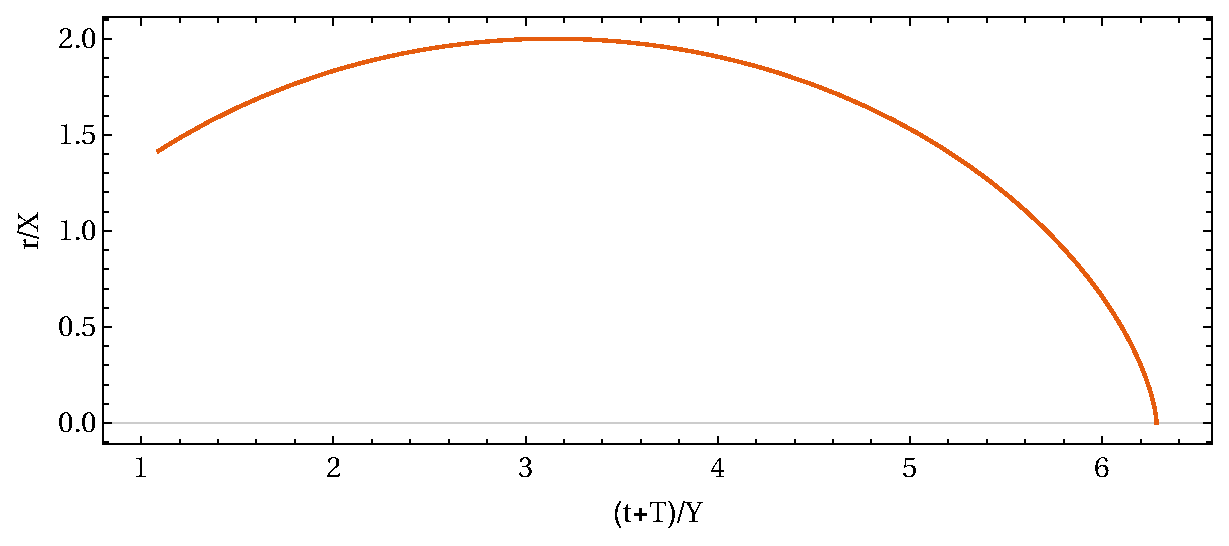
\includegraphics[width=\textwidth]{spherical.eps}
			\caption{\footnotesize The temporal evolution of the radius of a spherically symmetric perturbation. The parameter $\Theta$ goes from an arbitrary initial point (2 in this case) to $2\pi$. Of course, if $\Theta$ were to exceed that, this would periodically repeat. One needs to take into account the pressure experienced by matter at larger densities to effectively halt the gravitational collapse.}
			\label{fig:sphere-cycloid}
		\end{figure}
		
		In these terms, the maximum radius would be $2X$ and thus 
		$$
		\begin{aligned}
			X&=\frac{r_i}{2}\frac{1+\delta_i}{1+\delta_i-\Omega_i^{-1}}\\
			Y&=\frac{1+\delta_i}{2H_i\Omega_i^{1/2}	(1+\delta_i-\Omega_i^{-1})^{3/2}}
		\end{aligned}
		$$
		\subsection{Flat background universe}
			In this case, the equations are simplified on the account of $\Omega_i=1$. Thus,
			$$
			\begin{aligned}
				r&=\frac{r_i}{2}\left(\frac{1+\delta_i}{\delta_i}\right)(1-\cos\Theta)\\
				t+T&=\frac{1}{2H_i}\frac{1+\delta_i}{\delta_i^{3/2}}(\Theta-\sin\Theta)\\
			\end{aligned}
			$$
			At $t=t_i$, $\cos\Theta_i=(1-\delta_i)/(1+\delta_i)$. Going by our assumption that $\delta_i\ll 1$, $\cos\Theta_i\approx1-2\delta_i$. Or $\Theta_i^2\approx4\delta_i$. This means
			$$
				H_i(t_i+T)=\frac{2}{3}(1+\delta_i)
			$$
			Since the background universe in a  matter dominated context obeys $H_it_i=2/3$, it follows that $T=2\delta_i/3H_i$ or $T/t_i=\delta_i\ll1$.
			
			To understand the evolution of the density contrast, one must understand the evolution of the background density as well. In the matter dominated universe,
			\begin{equation}
				\begin{aligned}
					a\propto t^{2/3}; \rho_b&=\frac{1}{6\pi G t^2}\\
					\therefore 1+\delta=\frac{\rho}{\rho_b}&=\frac{3M}{4\pi X^3}\frac{6\pi GY^2(\Theta-\sin\Theta)^2}{(1-\cos\Theta)^2}\\
					\delta&=\frac{9(\Theta-\sin\Theta)^2}{2(1-\cos\Theta)^3}-1\\
				\end{aligned}
			\end{equation}
			In the low $\Theta$ limit,
			$$
				\begin{aligned}
					\delta&=\frac{9}{2}\frac{(\frac{\Theta^3}{3!}-\frac{\Theta^5}{5!}+\mathcal{O}(\Theta^7))^2}{(\frac{\Theta^2}{2!}-\frac{\Theta^4}{4!}+\mathcal{O}(\Theta^6))^3}-1\\
					&=\left(1-\frac{\Theta^2}{10}+\mathcal{O}(\Theta^4)\right)\left(1+\frac{\Theta^2}{4}+\mathcal{O}(\Theta^4)\right)-1\\
					&=\frac{3\Theta^2}{20}+\mathcal{O}(\Theta^4)\\
					t&=\frac{Y\Theta^3}{6}+\mathcal{O}(\Theta^5)\\
					\therefore \delta&\approx\frac{3}{20}\left(\frac{6t}{Y}\right)^{2/3}\\
				\end{aligned}
			$$
			Since $H_i=2/(3t_i)$ for a flat, matter dominated universe,
			$$
				\delta=\delta_i\left[\frac{3}{5}\left(\frac{t}{t_i}\right)^{2/3}\right]\propto a
			$$
			This is exactly what one would get if one were to pop $H=2/(3t)$ in \ref{eq:growth-linear}. Thus this is consistent with the linear solution in the case where there is no peculiar velocity.
			
			$t/Y=2\pi$ corresponds to the case when the spherical overdensity collapses to a single point. This put in the expression for $\delta$ in the linear limit yields $\delta\approx1.69$. This defines a density scale for collapse.
			
		\subsection{Virialisation}
			It can be estimated that the density contrast at turn-around would be nearly 4.6. This clearly lies in the non-linear regime. Now of course, the overdensity won't collapse to a singularity because the assumption that the peculiar velocities are negligible would break down at some point and this would mean the matter would exert a counter-acting pressure and the matter would come to an equilibrium.
			
			Equilibrium is reached via a process known as violent relaxation. This requires scattering of particles around small scale fluctuations and reach virial equilibrium in essentially the dynamical timescale, i.e. the time it takes for a particle to cross the spherical overdensity.
			
			One can compute something called the virial velocity and virial radius, which are defined through the energy equation at virial equilibrium. When the perturbation reached its maximum radius, all energy was in the form of potential energy. At virial equilibrium,
			$$
				\begin{aligned}
					K&=-\mathcal{E}\\
					 &=\frac{3GM^2}{5r_m}\\
				   2K&=-U\\
				   Mv_{vir}^2&=\frac{3GM}{5r_{vir}}\\
					v_{vir}=\left(\frac{6GM}{5r_m}\right)^{1/2}&;
					r_{vir}=r_m/2\\
				\end{aligned}
			$$
			Once the system is virialised, its density doesn't change and the density contrast simply evolves due to the background expansion. The density is:
			$$
				\rho_{coll}\approx 2^3\rho_m=8\times5.6\rho_b(t_{m})=170\rho_b(t_{coll})\\
			$$
	\section{Press-Schechter Formalism}
		In the conventional (by the standards of 1973) theory of cosmological perturbations,	structures arose from condensations of mass from large lengthscales. That is, mass aggregates on larger length scales before gravitation took it further and made denser and denser objects: Large clouds condensed to small clouds and yet smaller ones. While this seems to explain the formation of large objects of the order of $10^{15}M_\Sun$ and not on the scales of stars.
		
		The way out of this proposed by Zeldovich et al. was to develop non-linear, pancake-like structures that then developed shocks and fragmented to form lumpier objects.
		
		Press and Schechter in their 1973 paper proposed a bottom up approach, citing the possibility of statistical fluctuations of matter density growing in size due to self gravitation. That is, starting from point masses, fluctuations could grow in size due to matter aggregating. What they obtained as a result was the distribution of objects with a mass in the range $[M, M+dM]$.
		
		We saw in the previous section that density contrast of $1.69$ or higher leads to gravitational collapse. Press-Schechter formalism predicts the fraction of the volume that has collapsed as:
		\begin{equation}
			f_{coll}(M(R),z)=\int_{\delta_c}^{\infty}\frac{2}{\sqrt{2\pi}\sigma(R,z)}e^{-\delta^2/2\sigma^2(R,z)}d\delta\\
			\label{eq:Press-Schecht-fract}
		\end{equation}
		This requires some explanation. Firstly, one must realise not all length-scales are similar when it comes to collapse statistics. The easiest way of seeing that is by considering a density distribution and smoothing it over a window. 
		$$
			\delta(\mathbf{x},R)=\int \delta(\mathbf{x'})W(\mathbf{x-x'},R)d^3x
		$$
		Many peaks that previously appeared over the critical value will now be below it or are smoothed out to form fewer peaks. Thus it appears as if more clumps will form on the lower lengthscale but they will be less massive.
		The process of smoothing is merely a convolution with a window function $W$. This is represented rather simply as a product in the Fourier space:
		$$
			\delta(\mathbf{k},R)=\delta(\mathbf{k})\tilde{W}(kR)
		$$
		The functional dependence of $\tilde{W}$ on $R$ is made explicit in the statement above. It appears specifically as a product $kR$.
		In \ref{eq:Press-Schecht-fract}, $R$ is the radius of the smoothing window. $M$ is the mass enclosed within. 
		$$
			M=\gamma_f\bar{\rho}R^3\\
		$$
		Where $\bar{\rho}$ is the density averaged over the volume of the window and $\gamma_f$ is a constant that depends on the shape of the window function. $W$ is normalised such that its integral is 1 over the volume of integration. For example, $\gamma_f=4\pi/3$ for a top hat profile (constant within the spherical window but 0 outside).
		The  variance of the Gaussian integrand is a function of this radius and also the redshift of interest. Specifically, it is defined as the variance of the smoothed linear power spectrum. 
		$$
			\begin{aligned}
				\sigma^2&=\frac{1}{(2\pi)^3}\int P_{lin}(k)\tilde{W}^2(kR)d^3k\\
				&=\frac{1}{(2\pi)^2}\int P_{lin}(k)\tilde{W}^2(kR)k^2dk
			\end{aligned}
		$$
		Of course, there is implicit dependence of redshift in $P_{lin}$ and hence $\sigma$. Now one can define the window function in terms of either the radius or the mass enclosed. So in terms of mass, the variance can be written as:
		$$
			\sigma^2_M=\Big\langle\left(\frac{M(\mathbf{x},R)-\bar{M}}{\bar{M}}\right)^2\Big\rangle
		$$
		Where the $M$ is the density convolved with the window function and multiplied by the window volume. $\bar{M}$ is the aveagre of $M$ over that volume. 
		Thus, given a particular redshift and a particular window, the fraction of volume that collapses is given by \ref{eq:Press-Schecht-fract}. Now this expression needs to be examined more carefully.
		\begin{enumerate}
			\item Now it is highly dubious that the distribution of inhomogeneities is Gaussian. This is simply because $\delta>-1$. Even if the mean were high and one could \emph{approximate} the distribution to be Gaussian, evolution under the influence of gravity would produce a lot of underdense regions and a significant tail of overdense regions. 
			\item The normalisation itself is questionable because of the factor of two in the numerator.
			\item The proposed form of $\sigma$ ignores non-linear effects. There is a huge disagreement in its value obtained from the linear power-spectrum as compared to the true non-linear one.
		\end{enumerate}
		With all these points to be sceptic about, it is surprising that the formalism produces great numerical results regarding clustering. The factor of two in the normalisation was introduced as a fudge factor by Press and Schechter. Without this factor, the theory would predict that only half the mass of the universe would be locked up in haloes. There were more attempts to explain theoretically as to why the P-S formalism works so well.
		
		Another way of expressing \ref{eq:Press-Schecht-fract} is in terms of number density of objects within a given mass range $[M,M+dM]$.
		\begin{equation}
			\begin{aligned}
				\frac{dn}{dM}&=-\frac{\rho_m}{M}\frac{df_{coll}}{dM}\\
				&=-\frac{\rho_m}{M}\frac{df_{coll}}{d\sigma}\frac{d\sigma}{dM}\\
				&=-\frac{\rho_m}{M}\frac{d\sigma}{dM}\frac{d}{d\sigma}\int_{\delta_c}^{\infty}\frac{2}{\sqrt{2\pi}\sigma(R,z)}e^{-\delta^2/2\sigma^2(R,z)}d\delta\\
				&=-\sqrt{\frac{2}{\pi}}\frac{\rho_m}{M}\frac{d\sigma}{dM}\frac{\delta_c}{\sigma^2}e^{\delta_c^2/2\sigma^2}\\
				&=-\sqrt{\frac{2}{\pi}}\frac{\rho_m\delta_cR}{3M^2\sigma^2}\frac{d\sigma}{dR}e^{\delta_c^2/2\sigma^2}\\
			\end{aligned}
		\end{equation}
		Here $\rho_m/M$ is the average number density of such objects. The negative signature essentially signifies the increasing rarity of more massive objects. The last equation uses the fact that $dM/dR = 3M/R$.
		
		Now the critical density was calculated to be 1.69 for the case of the spherically symmetric model. If one were to perform numerical simulations and find out this value by keeping it a free parameter, it would turn out ot be pretty close to 1.69.  
\end{document}